%%%%%%%%%%%%%%%%%%%%%%%%%%%%%%%%%%%%%%%%%%%%%%%%%%%%%%%%%%%%%%%%%%%%%%%%%%% 
% 
% Generic template for TFC/TFM/TFG/Tesis
% 
% $Id: introduccion.tex,v 1.22 2020/03/24 17:18:20 macias Exp $
% 
% By:
% + Javier Macías-Guarasa. 
% Departamento de Electrónica
% Universidad de Alcalá
% + Roberto Barra-Chicote. 
% Departamento de Ingeniería Electrónica
% Universidad Politécnica de Madrid   
% 
% Based on original sources by Roberto Barra, Manuel Ocaña, Jesús Nuevo,
% Pedro Revenga, Fernando Herránz and Noelia Hernández. Thanks a lot to
% all of them, and to the many anonymous contributors found (thanks to
% google) that provided help in setting all this up.
% 
% See also the additionalContributors.txt file to check the name of
% additional contributors to this work.
% 
% If you think you can add pieces of relevant/useful examples,
% improvements, please contact us at (macias@depeca.uah.es)
% 
% You can freely use this template and please contribute with
% comments or suggestions!!!
% 
%%%%%%%%%%%%%%%%%%%%%%%%%%%%%%%%%%%%%%%%%%%%%%%%%%%%%%%%%%%%%%%%%%%%%%%%%%% 

\chapter{Introducción}
\label{cha:introduccion}

\begin{FraseCelebre}
  \begin{Frase}
    Desocupado lector, sin juramento me podrás creer que quisiera que este
    libro [...] fuera el más hermoso, el más gallardo y más discreto que
    pudiera imaginarse\footnote{Tomado de ejemplos del proyecto \texis{}.}.
  \end{Frase}
  \begin{Fuente}
    Miguel de Cervantes, Don Quijote de la Mancha
  \end{Fuente}
\end{FraseCelebre}


\section{Presentación}
\label{sec:presentacion}


Esta plantilla\footnote{Asegúrate de compilar de nuevo el documento
  (como cuenta la sección~\ref{sec:compilacion}), para verificar que
  todo funciona y por si ha habido algún cambio en los fuentes que no
  está reflejado en los pdf de ejemplo precompilados.} pretende
proporcionar un conjunto de estilos consistentes y unificados para
cubrir las necesidades de generación de memorias \LaTeX{} para cada uno
de los TFCs/TFMs/TFGs y tesis doctorales que se generen en la Escuela
Politécnica Superior de la Universidad de Alcalá\footnote{También se
  incluye la definición para las tesis de la Escuela Técnica Superior de
  Ingenieros de Telecomunicación de la Universidad Politécnica de
  Madrid. La extensión a los TFGs de la misma es sencilla, aunque no se
  ha realizado por el momento.}.

Para utilizar la plantilla se han generado algunos capítulos genéricos
en los que se han incluido secciones ``tutoriales'', en la que se
explican algunas de sus características y se muestran ejemplos de
elementos típicos que pueden ser de utilidad (pero sin el objetivo de
que esto sea una guía de \LaTeX{}).

Igualmente se proporciona un modelo simplificado de un anteproyecto
(para el caso de los TFCs/TFMs/TFGs), así como parte de la documentación
que hay que presentar para la defensa de los TFGs/TFMs de la Universidad
de Alcalá.



\section{Uso de la plantilla}
\label{sec:uso-generico-de}


\subsection{Prerrequisitos}
\label{sec:prerrequisitos}

Para usar la plantilla tal y como está definida, hace falta disponer de
una serie de paquetes de estilos \LaTeX{} (ficheros \texttt{.sty}),
todos ellos definidos en el fichero \texttt{Config/preamble.tex}.

No vamos a hacer un listado de todos lo necesarios (sería demasiado
largo\footnote{Los que suelen no estar instalados en un ubuntu estándar
  son \texttt{texlive-publishers}, \texttt{texlive-science}}), pero en
la mayoría de distribuciones GNU/Linux serán fáciles de conseguir en
caso de que la compilación genere un error de fichero no encontrado. Si
os sucede, buscadlos en alguno de los paquetes \texttt{texlive-*}. En
caso de no encontrarlos, una búsqueda en google (que con casi total
seguridad referenciará a alguna página en CTAN) os dará el enlace a la
descarga correspondiente. A partir de ahí, su inclusión en directorios
locales será suficiente.
% (como por ejemplo hemos tenido que hacer con el
% paquete \texttt{background}, incluido en la distribución en el
% directorio \texttt{sty/background}). Lo más cómodo es hacer una
% instalación del \texttt{texlive-full}. 

Igualmente será necesario tener instaladas una serie de utilidades y
aplicaciones:

\begin{itemize}
\item En Linux

  \begin{itemize}
  \item \texttt{make}, si se quiere utilizar la facilidad del
    \texttt{Makefile} suministrado. Está disponible en todas las
    distribuciones GNU/Linux.
  \item \texttt{rubber}, si se quiere utilizar la prestación de
    compilación de código \LaTeX{} incluida en el
    \texttt{Makefile}. Debería estar disponible en cualquier distribución
    GNU/Linux, pero si no es así, puedes optar por descargarla, o bien
    usar la alternativa de \texttt{latexmk} (para el que también se
    incluyen targets específicos en el \texttt{Makefile} suministrado).
  \item \texttt{dia}, si se quiere utilizar el ejemplo proporcionado de
    generación de esquemas con dicha herramienta.
  \item \texttt{epspdf}, si se quiere utilizar la facilidad de la
    conversión automática de ficheros \texttt{eps} a \texttt{pdf} (también
    se usa en la conversión de ficheros \texttt{.dia}).
  \item \texttt{makeglossaries}, si se quiere utilizar la prestación de
    manejo de listas de acrónimos y variables. Suele estar en el paquete
    \texttt{texlive-latex-extra} en distribuciones basadas en Debian
    (como ubuntu y derivados).
  % \item \texttt{latexdiff} y \texttt{latexpand}, si se quiere utilizar la
  %   prestación de generación de ficheros pdf con control de cambios. El
  %   primero suele ser un paquete independiente, y el segundo suele estar
  %   en el paquete \texttt{texlive-extra-utils}.
  \end{itemize}

\item En Windows (os cuento la configuración que he probado en algún momento):

  \begin{itemize}
  \item \texttt{miktex} como sistema de compilación \LaTeX{}, diciéndole
    que instale todo lo que necesite.
  \item \texttt{TeXstudio} o \texttt{TeXMaker} como editor.
  \item Para usar glossaries, echadle un ojo a
    \url{https://tex.stackexchange.com/questions/156270/has-anyone-managed-to-use-glossaries-with-texstudio-on-windows}. Os
    copio aquí info que nos han pasado al respecto (gracias Cristina
    Losada): En Texmaker se puede configurar la “Compilacion rápida”
    con los comandos que queramos. Eso está en el menú Opciones a
    Configurar Texmaker, y a la izquierda de la ventana que sale hay
    que elegir “Compilación rápida”. Hay las opciones típicas, y
    además permite usar los comandos elegidos por el usuario. Ahí yo
    tengo esta configuración (compila con pdflatex, llama además a
    bibtex y makeglossaries y al final muestra el pdf):
    \texttt{pdflatex -synctex=1 -interaction=nonstopmode \%.tex|bibtex \%|makeglossaries \%|pdflatex -synctex=1 -interaction=nonstopmode \%.tex|pdflatex -synctex=1 -interaction=nonstopmode \%.tex|}''\texttt{C:/Program Files (x86)/Adobe/Acrobat Reader DC/Reader/AcroRd32.exe}''\texttt{ \%.pdf}
  \item \texttt{make}, si se quiere utilizar la facilidad del
    \texttt{Makefile} suministrado. Hay varias opciones y que necesita
    un intérprete de comandos (es posible que con el nuevo WSL sea más
    fácil todavía).
  \end{itemize}
\end{itemize}

\subsection{Compilación}
\label{sec:compilacion}

Para facilitar la generación del documento se incluye un
\texttt{Makefile} relativamente sencillo. No somos expertos ni en
\texttt{make} ni en \LaTeX, con lo que seguro que no es el mejor de los
\texttt{Makefiles} del mundo, pero creemos que hace su función.

El \texttt{Makefile} tiene las siguientes características y
prestaciones:

\begin{itemize}

\item Hace uso de la herramienta \texttt{rubber}. En caso de no disponer
  de ella, puede usarse \texttt{latexmk} (hay targets específicos de
  ejemplo para ese caso), pero esta última herramienta no ha sido
  probada intensivamente. Si no se dispone de ninguna de ellas, habría
  que generar la estructura típica de compilación: (al estilo
  \texttt{pdflatex + bibtex + pdflatex + pdflatex}).
\item Soporta la generación automática de ficheros \texttt{pdf} a partir
  de los \texttt{dia} y \texttt{svg} (se han elegido estos a modo de
  ejemplo, pero se puede adaptar fácilmente a otras necesidades).
\item Genera la información de listas de acrónimos y símbolos con la
  herramienta \texttt{makeglossaries}. Es imprescindible tenerla
  instalada si se desea usar esa capacidad.
\item Soporta los targets:
  \begin{itemize}
  \item \texttt{all} (que es la opción predeterminada si se ejecuta
    \texttt{make} sin más argumentos), que genera el fichero
    \texttt{book.pdf} correspondiente, usando \texttt{rubber} y
    \texttt{makeglossaries}. No nos hemos planteado la generación de
    ficheros en otros formatos.
  \item \texttt{all\_latexmk}, que genera el fichero \texttt{book.pdf}
    correspondiente, usando \texttt{latexmk} y
    \texttt{makeglossaries}. Si ésta  es tu opción, sustituye el target
    \texttt{all} por éste, para facilitarte la compilación.

  \item  \texttt{tar}, que genera un fichero \texttt{tgz} que contiene
    todo lo necesario para la distribución de la plantilla.
  \item \texttt{clean}, que borra todos los ficheros temporales usando
    \texttt{rubber} (para simplificar los targets, la limpieza se hace
    tanto para los temporales de generación del \texttt{book.pdf} como
    los del \texttt{anteproyecto.pdf}).
  \item \texttt{clean\_latexmk}, que borra todos los ficheros temporales
    usando \texttt{latexmk}. Si ésta es tu opción, sustituye el target
    \texttt{clean} por éste, para facilitarte la compilación (para
    simplificar los targets, la limpieza se hace tanto para los
    temporales de generación del \texttt{book.pdf} como los del
    \texttt{anteproyecto.pdf}).

  \item \texttt{bare}, que deja razonablemente limpios los ficheros de
    los capítulos y apéndices, además de borrar los gráficos del
    directorio \texttt{figures} y \texttt{diagrams}, para que sea más
    fácil comenzar a editar. \textbf{OJO: HAY CONSECUENCIAS NEGATIVAS NO
      DESPRECIABLES PORQUE SE BORRARÁ TODO LO QUE TENGAS EN ESOS
      DIRECTORIOS Y SÓLO DEBERÍA HACERSE CUANDO VAYAMOS A EMPEZAR A
      ESCRIBIR NUESTRA MEMORIA DEL TRABAJO REALIZADO}.

  \item \texttt{backup-chapters}, que hace un backup de los ficheros que
    hay en los directorios \texttt{chapters} y \texttt{appendix},
    creando directorios cuyo nombre es la fecha y hora actuales y que se
    crean bajo los anteriores. No debería hacer falta si usas un buen
    sistema de control de versiones.
  \end{itemize}

\end{itemize}


\subsection{Detalles específicos para sistemas basados en MacOS}
\label{sec:detall-espec-para}

Esta información es cortesía de Carlos Cruz, que se encontró con un
problema en la generación de la lista de acrónimos. Copio a
continuación los detalles al respecto.

Hemos encontrado que la lista de acrónimos y/o símbolos no se genera en
el entorno macOS. Recomendamos seguir las siguientes instrucciones para
solucionar este problema:

\begin{itemize}
\item Tener el SO actualizado a la última versión. Actualmente (marzo de
  2020) MacOS Catalina versión 10.15.2
\item Instalar la última versión de MacTeX-2019. Esta distribución
  requiere Mac OS 10.12, Sierra, o superior y funciona con procesadores
  Intel (disponible en
  \href{http://tug.org/mactex/mactex-download.html}{http://tug.org/mactex/mactex-download.html}).
\item Trabajar en el entorno Texshop version 4.44:
  \href{https://pages.uoregon.edu/koch/texshop/}{https://pages.uoregon.edu/koch/texshop/}.
\end{itemize}

Si compilamos la plantilla en el entorno Texshop, comprobamos que los
listados de glosario y/o símbolos no se compilan con ninguno de los
Typeset: Latex, Lualatex, Xelatex o pdflatexmk.

Recomendamos inicialmente compilar por Terminal:

\begin{itemize}
\item pdflatex “nombre del fichero.tex” (compilar dos veces)
\item makeglossaries “nombre del fichero”
\item pdflatex “nombre del fichero” (compilar dos veces)
\end{itemize}

De esta forma, se crea correctamente la lista de acrónimos y símbolos. A
continuación, se puede trabajar con futuros cambios en el proyecto
mediante Texshop compilando Latex. Si quiere actualizar o modificar la
lista de acrónimos y/o símbolos nuevamente, recomendamos borrar todos
los ficheros salvo el fichero book.tex y compilar de nuevo por consola
para crear la lista correctamente.



\subsection{Estructura del documento generado por la plantilla}
\label{sec:estr-del-docum}

La plantilla definida presenta la siguiente estructura:

\begin{itemize}

\item Portada y página de información sobre el trabajo, que será
  dependiente del tipo de trabajo y la titulación. Se genera
  automáticamente a partir de la información definida en la
  sección~\ref{sec:definicion-del-tipo}

\item Ficheros pdf insertados, que aplican en algunos de los tipos de
  documentos (por ejemplo en las tesis doctorales).

\item Dedicatoria, con un ejemplo incluido en el fichero
  \texttt{dedication/dedicatoria.tex}.
\item Agradecimientos, con un ejemplo incluido en el fichero
  \texttt{dedication/agradecimientos.tex}.


\item Resumen en español, con un ejemplo incluido en el fichero
  \texttt{abstract/resumen.tex}.
\item Resumen en inglés, con un ejemplo incluido en el fichero
  \texttt{abstract/abstract.tex}.
\item Resumen extendido en español (opcional en algunos tipos de
  documento), con un ejemplo incluido en el fichero
  \texttt{abstract/resumen-extendido.tex}.

\item Índice de contenidos, índice de figuras e índice de tablas.
\item Índices adicionales, de los que se incluye un ejemplo de listado
  específico en el fichero \texttt{cover/extralistings.tex}, que incluye
  el listado de fragmentos de código fuente definidos en el
  \texttt{appendix/manual.tex}.

\item Listado de acrónimos utilizados, que se definen en el fichero
  \texttt{acronyms/defacronymsgl.tex} (con opciones adicionales de
  configuración en \texttt{acronyms/acronymsgl.tex}), y del que
  incluimos más información en la sección~\ref{sec:uso-de-acronimos}.
\item Listado de símbolos utilizados, que se definen en el fichero
  \texttt{symbols/defsymbolsgl.tex} (con opciones adicionales de
  configuración en \texttt{symbols/symbolsgl.tex}), y del que incluimos
  más información en la sección~\ref{sec:simbolos}.


\item Capítulos del documento, del que hay varios ejemplos que siguen la
  estructura típica (introducción, estudio teórico, desarrollo,
  resultados y conclusiones.

\item Pliego de condiciones y presupuesto, opcionales en función del
  tipo de documento que se genere (se incluyen un
  par de ejemplos del trabajo fin de carrera de Jesús Martínez en los
  ficheros \texttt{pliego/pliego-ejemplo.tex} y
  \texttt{presupuesto/presupuesto-ejemplo.tex}. Es un trabajo antiguo y
  es necesario que busquéis esquemas y contenidos actualizados para
  estos capítulos.

\item Bibliografía, de la que se puede cambiar el estilo utilizado y los
  ficheros \texttt{.bib} en el fichero
  \texttt{biblio/bibliography.tex} (en el que hay que definir la lista
  de ficheros de bibliografía que se usarán (variables
  \texttt{\textbackslash{}mybibfileOne},
  \texttt{\textbackslash{}mybibfileTwo}, ...).

\item Apéndices, de los que ahora se incluyen dos ejemplos en los
  ficheros \texttt{appendix/manual.tex} (que sirve de pretexto para
  mostrar cómo se insertan fragmentos de código fuente), y
  \texttt{appendix/herramientas.tex}.
\item Contraportada.
\end{itemize}

Por supuesto, modificad la estructura para que encaje en las directrices
que tengáis al respecto de cómo documentar vuestro trabajo.


\subsection{Definiciones específicas del tipo de documento}
\label{sec:definicion-del-tipo}

Para comenzar a usar la plantilla es fundamental revisar el fichero
\texttt{book.tex} en el que se incluyen todos los detalles genéricos de
la estructura usada en el documento, con comentarios que esperamos que
os ayuden a entenderlo. Si sois de los impacientes, basta con que
comencéis por la parte en la que se incluyen los distintos capítulos
(buscad la parte de los \texttt{\textbackslash{}input\{chapters/*.tex\}}).

El fichero de configuración más importantes es el
\texttt{Config/myconfig.tex} en el que se incluyen elementos para
determinar la configuración específica de tu documento y que es de
donde se toman los datos para las muchas automatizaciones del proceso
de generación. El primero de ellos (para facilitar la generación de
documentos en español o inglés), es el que define el idioma que vas a
utilizar. Para seleccionarlo, basta con asignar \texttt{spanish} o
\texttt{english} a la variable \texttt{\textbackslash{}myLanguage}. A
partir de ella, el sistema generará las cabeceras y títulos adecuados
a cada una.

Igualmente, tendréis que definir las siguientes variables sobre el tipo
de trabajo y el autor:

\begin{itemize} 
\item Acrónimo de la titulación correspondiente al trabajo (variable
  \texttt{\textbackslash{}myDegree}): Que se seleccionará entre los
  definidos (por ahora\footnote{Este apartado se generó en marzo de
    2020.} son \texttt{IT}, \texttt{IE}, \texttt{ITTSE}, \texttt{ITTST},
  \texttt{ITI}, \texttt{GIEC}, \texttt{GIST}, \texttt{GITT},
  \texttt{GIT}, \texttt{GIEAI}, \texttt{GITI}, \texttt{GIC},
  \texttt{GII}, \texttt{GSI}, \texttt{GISI}, \texttt{MUSEA},
  \texttt{MUIT}, \texttt{MUII}, \texttt{PHDUAH} y \texttt{PHDUPM}) y que
  automáticamente configura portadas\footnote{Un comentario sobre el
    color de las bandas en la portada de los TFGs: de acuerdo con la
    normativa, dicho color debe ser PANTONE 160c. Yo he intentado
    utilizar dicho color, pero el aspecto con el que finalmente aparece
    no es ni de lejos similar al del modelo que proporciona la EPS, con
    lo que he optado por utilizar el que se ve realmente en dicho
    modelo. Si quieres cambiarlo, busca ``PANTONE'' en
    \texttt{Config/preamble.tex}.}, entre otras cosas.

\item Flag de división de directores (variable
  \texttt{\textbackslash{}myFlagSplittedAdvisors}). Si puesta a
  \texttt{false} indicará ``Tutores/Advisors'' en las páginas de
  portada. En caso contrario lo separará en líneas para
  ``Tutor/Advisor'' y ``Cotutor/Co-Advisor''.

\item Especialidad (nuevo en TFGs desde el curso 2015) (variable
  \texttt{\textbackslash{}mySpecialty})

\end{itemize}

Sobre el documento en general:

\begin{itemize}
\item Título del documento en español (variable
  \texttt{\textbackslash{}myBookTitleSpanish}).
\item Título del documento en inglés (variable
  \texttt{\textbackslash{}myBookTitleEnglish}).
\item Palabras clave en inglés (variable \texttt{\textbackslash{}myThesisKeywordsEnglish}).
\item Palabras clave en español (variable \texttt{\textbackslash{}myThesisKeywords}).


\end{itemize}

Sobre el autor y el tutor y cotutor:

\begin{itemize}
  
\item Nombre del autor del trabajo (variable
  \texttt{\textbackslash{}myAuthorName}).
\item Apellidos del autor del trabajo (variable
  \texttt{\textbackslash{}myAuthorSurname}). La unión de esta
  definición con la del nombre formará automáticamente la variable
  \texttt{\textbackslash{}myAuthorFullName}
\item Género del autor (variable
  \texttt{\textbackslash{}myAuthorGender}), ``male'' or ``female''.
\item Email del autor (variable
  \texttt{\textbackslash{}myAuthorEmail}).
\item DNI del autor del trabajo, usado en el papeleo de los TFGs
  (variable \texttt{\textbackslash{}mybookDNI}).

\item También se ha iniciado soporte básico para generar la hoja de
  control de anteproyecto que se usa en la solicitud, con lo que hay
  variables relacionadas con los datos personales del alumno:

  \begin{itemize}
  \item Dirección: calle (variable \texttt{\textbackslash{}myAuthorStreet}),
    ciudad (variable \texttt{\textbackslash{}myAuthorCity}), código postal
    (variable \texttt{\textbackslash{}myAuthorPostalCode}), provincia (variable
    \texttt{\textbackslash{}myAuthorProvince}) y teléfono (variable
    \texttt{\textbackslash{}myAuthorTelephone}).
  \end{itemize}

\item Nombre del primer (o único, en su caso) director/tutor del trabajo
  (variable \texttt{\textbackslash{}myAcademicTutorFullName}).
\item Género del primer director/tutor (variable
  \texttt{\textbackslash{}myAcademicTutorGender}), ``male'' or
  ``female''.
\item DNI del primer direector, para los permisos de publicación en
  abierto (variable \texttt{\textbackslash{}myFirstAdvisorDNI}

  
\item Nombre del segundo (en su caso) director/tutor del trabajo (variable
  \texttt{\textbackslash{}myCoTutoroFullName}).
\item Género del segundo director/tutor (variable
  \texttt{\textbackslash{}myCoTutorGender}), ``male'' or
  ``female''.
\item DNI del segundo director, para los permisos de publicación en
  abierto (variable \texttt{\textbackslash{}mySecondAdvisorDNI}), en
  su caso

  \end{itemize}

Sobre la filiación del autor y el trabajo:

\begin{itemize}

\item Centro en el que se realiza el trabajo (variable
  \texttt{\textbackslash{}mySchool}, que debería ser la Escuela
  Politénica Superior, pero se incluye por generalidad).
\item Universidad en el que se realiza el trabajo (variable
  \texttt{\textbackslash{}myUniversity}, que debería ser la de
  Alcalá, pero se incluye por generalidad).
\item Acrónimo de la Universidad (variable
  \texttt{\textbackslash{}myUniversityAcronym}).

\item Departamento en el que se realiza el trabajo (variable
  \texttt{\textbackslash{}myDepartment}, en español, y
  \texttt{\textbackslash{}myDepartmentEnglish}, en inglés).
  
\item Programa de Doctorado (en su caso) en el que se realiza el
  trabajo (variable \texttt{\textbackslash{}myPhDProgram}, en español,
  y \texttt{\textbackslash{}myPhDProgramEnglish}, en inglés).
\item Grupo de investigación en el que se realiza el trabajo (variable
  \texttt{\textbackslash{}myResearchGroup}.

  \end{itemize}

Sobre el tribunal:

\begin{itemize}

\item Nombre del presidente del tribunal (variable
  \texttt{\textbackslash{}myTribunalPresident}).
\item Nombre del primer vocal del tribunal (variable
  \texttt{\textbackslash{}myTribunalFirstSpokesperson}).
\item Nombre del segundo vocal del tribunal (variable
  \texttt{\textbackslash{}myTribunalSecondSpokesperson}).
\item Nombre del suplente del tribunal (variable
  \texttt{\textbackslash{}myTribunalAlternateMember}).
\item Nombre del secretario del tribunal, en su caso (variable
  \texttt{\textbackslash{}myTribunalSecretary}).
\item Nombre del Secretario del Departamento (que firmará parte del
  papeleo) (variable \texttt{\textbackslash{}myDepartmentSecretary}).

\end{itemize}

Sobre fechas varias:

\begin{itemize}
  
\item Fecha del anteproyecto, en su caso (variable
  \texttt{\textbackslash{}myThesisProposalDate}), en el caso de que se
  use la plantilla del anteproyecto
\item Fecha del anteproyecto en inglés, en su caso (variable
  \texttt{\textbackslash{}myThesisProposalDateEnglish}), en el caso de
  que se usen la plantilla del anteproyecto.

\item Fecha del depósito del trabajo (variable
  \texttt{\textbackslash{}myThesisDepositDate})
\item Fecha del depósito del trabajo en inglés (variable
  \texttt{\textbackslash{}myThesisDepositDateEnglish})

\item Año del trabajo (variable
  \texttt{\textbackslash{}myThesisDefenseYear}).
\item Fecha de la defensa del trabajo, en su caso (variable
  \texttt{\textbackslash{}myThesisDefenseDate}, en español, o
  \texttt{\textbackslash{}myThesisdefenseDateEnglish} en inglés).

\item Fecha que aparecerá en la firma del papeleo (variable
  \texttt{\textbackslash{}myPaperworkDate}).
  
\item Nombre del vicerrector (variable
  \texttt{\textbackslash{}myResearchVicerrector}).
\item Género del vicerrector (variable
  \texttt{\textbackslash{}myResearchVicerrectorGender}).
\end{itemize}

Se ha comenzado a trabajar en la versión alfa del soporte para
\textit{research reports}, y en ese caso se usa la variable
\texttt{\textbackslash{}myResearchReportID}.

Y también hay otras variables de menor interés o en desuso en las que
no vamos a entrar.

Parte de esa información se utilizará para rellenar la metainformación
incluida en el fichero \texttt{pdf} que se genera.


También se definen los colores que se usarán en los hiperenlaces del
documento:

\begin{itemize}
\item Color de los enlaces en el índice de contenidos (variable
  \texttt{\textbackslash{}mytoclinkcolor}).
\item Color de los enlaces en el índice de figuras (variable
  \texttt{\textbackslash{}myloflinkcolor}).
\item Color de los enlaces en el índice de tablas (variable
  \texttt{\textbackslash{}mylotlinkcolor}).
\item Color de los enlaces en otros índices (variable
  \texttt{\textbackslash{}myothertoclinkcolor}), de los que ahora se
  incluye un ejemplo en el fichero \texttt{cover/extralistings.tex}.
\item Color de los enlaces (\texttt{\textbackslash{}ref}) en el
  documento (variable \texttt{\textbackslash{}mylinkcolor}).
\item Color de los enlaces a URLs (variable
  \texttt{\textbackslash{}myurlcolor}).
\item Color de los enlaces a referencias bibliográficas (variable
  \texttt{\textbackslash{}mycitecolor}).
\end{itemize}

Basta con que definas las variables correspondientes y la plantilla
generará automáticamente las portadas adecuadas a la normativa y usará
las definiciones específicas que hayas seleccionado.

Por si os hace falta, en \texttt{Config/postamble.tex} se definen
muchas variables relacionadas con el tipo de trabajo, la
personalización y adaptación a género y número en distintos
documentos, etc. Por ejemplo las variables
\texttt{\textbackslash{}myDegreefull} (igual a ``\myDegreefull'' en
esta compilación), \texttt{\textbackslash{}myWorkType} (igual a
``\myWorkType'' en esta compilación) y
\texttt{\textbackslash{}myWorkTypeFull} (igual a ``\myWorkTypeFull''
en esta compilación). Otro ejemplo sería el autor de contacto:
\contactauthor.

Importante para las tesis de UAH: si necesitáis incluir ficheros pdf
(los de autorización e informes de los tutores, por ejemplo), esta
plantilla lo permite: mirad los \texttt{\textbackslash{}includepdf} en
el \texttt{book.tex}.

\subsection{Plantilla de anteproyecto}
\label{sec:plantilla-de-anteproyecto}

Para el caso de los TFMs/TFGs/TFCs, se incluye una plantilla para
realizar el anteproyecto.

La plantilla se encuentra en el directorio \texttt{Anteproyecto}, y en
fichero \texttt{anteproyecto.tex} tenéis un ejemplo. El
\texttt{Makefile} genera automáticamente el \texttt{anteproyecto.pdf},
haciendo un \texttt{make} en ese directorio, y tiene targets similares a los
del \texttt{Makefile} del documento principal, incluyendo
\texttt{flatten} y \texttt{latexdiff}, con lo que también puede
generarse el fichero con control de cambios, tal y como se describe en
la sección~\ref{sec:control-de-cambios} (cambiando las referencias a
\texttt{book...} por \texttt{anteproyecto...}).

\subsection{Plantilla de hoja de control de anteproyecto}
\label{sec:plantilla-de-hoja-control-anteproyecto}

Para el caso de los TFMs/TFGs/TFCs, se incluye una plantilla de la hoja
de control de la solicitud del anteproyecto.

La plantilla se encuentra en el directorio \texttt{Papeleo/SolicitudTFGTFM/}, y en
fichero \texttt{solicitud.tex} tenéis un ejemplo. El
\texttt{Makefile} genera automáticamente el \texttt{solicitud.pdf},
haciendo un \texttt{make} en ese directorio, y tiene targets similares a los
del \texttt{Makefile} del documento principal, incluyendo
\texttt{flatten} y \texttt{latexdiff}, con lo que también puede
generarse el fichero con control de cambios, tal y como se describe en
la sección~\ref{sec:control-de-cambios} (cambiando las referencias a
\texttt{book...} por \texttt{solicitud...}). En este caso el documento
no hay que tocarlo prácticamente, salvo que le pase alguna cosa rara.


\subsection{Papeleo adicional}
\label{sec:introapp1}

Para el caso de los TFGs y TFMs se incluyen en el directorio
\texttt{papeleo} algunos de los documentos que hay que generar en el
momento de la defensa. En concreto:

\begin{itemize}
\item La autorización del tutor para la publicación en abierto, en el
  fichero
  \texttt{Papeleo/AutorizacionRepoInstit/autorizacionTutorPublicarRepositorio.tex}
  para TFGs.
\item La autorización del autor para la publicación en abierto, en el
  fichero
  \texttt{Papeleo/AutorizacionRepoInstit/autorizacionAutorPublicarRepositorio.tex}
\item El visto bueno del tutor para la defensa del TFG
  \texttt{Papeleo/TFG/vistoBuenoTutorTFG.tex}
\item La solicitud de acta para la defensa del TFG
  \texttt{Papeleo/TFG/solicitudActaTFG.tex}
\item El visto bueno del tutor para la defensa del TFM
  \texttt{Papeleo/TFM/vistoBuenoTutorTFM.tex}
\end{itemize}

En cada uno de esos directorios se incluye un \texttt{Makefile} que
genera los \texttt{pdfs} correspondientes a esos documentos. El
sistema automáticamente adapta los singulares/plurales necesarios para
el caso de que haya uno o varios directores/tutores.


\subsection{Generación del documento con control de cambios (para
  revisión)}
\label{sec:control-de-cambios}

Uno de los problemas de \LaTeX{} frente a otros sistemas de edición de
textos viene en el momento de la revisión de cambios realizados a un
documento. En el caso que nos ocupa serían los que nos sugiere nuestro
tutor de TFC/TFG/TFG o director de tesis doctoral y que luego querrá
verificar cómo se han aplicado. En un procesador al estilo de
libreoffice (vaaaaaaaaale, o Microsoft Word también), tenemos la opción
de comparar documentos o llevar el control de cambios y que el sistema
automáticamente nos marque los añadidos o borrados. 

En \LaTeX{} también es posible si usamos un sistema de control de
versiones (y si no lo estáis usando, deberíais plantearos seriamente el
hacerlo), con la ayuda de herramientas adicionales.

Hay varias soluciones disponibles, la mayoría basada en el uso de la
\texttt{latexdiff}~\cite{latexdiff} (o derivados). Lo recomendable
sería el uso de un sistema automatizado como el disponible en
\texttt{git-latexdiff} \cite{git-latexdiff}, pero necesita el soporte
de \texttt{git}, y dados los orígenes en los que mantenía esto en
\texttt{cvs} (flames to \texttt{/dev/null}, please), o pensando en los
que no usaréis ningún sistema de control de versiones (si es así, mal
hecho, por cierto, deberías usar alguno) el mecanismo que uso es un
poco más rupestre (si quieres ayudarme a generalizar esto, sería
perfecto).

\texttt{latexdiff} permite comparar dos versiones de un documento y
generar un nuevo fichero fuente en \LaTeX{} que, al compilarlo, muestra un
pdf  ``bonito'', con las marcas de las diferencias (resaltando lo añadido
y lo quitado). El resultado es perfecto para hacer una buena revisión de
los cambios, y por supuesto no tiene punto de comparación con ver un
\texttt{diff} a palo seco de las dos versiones del documento. 

Lo que finalmente he implementado es muy ad-hoc, pero
funciona\footnote{por algún motivo, a fecha de julio de 2021,
  \texttt{latexdiff} genera código erróneo, y he tenido que hacer una
  super ñapa en el \texttt{Makefile} para solucionarlo, así que en el
  futuro seguro que da problemas. Be warned!}.

El procedimiento para generar un documento que muestre las
diferencias es el siguiente (asumo disponible un intérprete de
comandos y la utilidad \texttt{make}):

\begin{itemize}
\item Primero hay que preparar la versión base sobre la que luego se
  harán los cambios. Esa preparación se hace normalmente cuando se
  tiene una versión razonablemente estable, y con la que luego se
  quiere comparar (por ejemplo cuando le entregas a tu tutor tu primer
  borrador del documento completo). La preparación es sencilla: basta
  hacer un \texttt{make snapshot}. Eso generará un fichero
  \texttt{book-flatten-snapshot.tex} que contiene el estado actual del
  documento, expandido. Lo suyo sería luego registrarlo en el
  repositorio con un \texttt{cvs commit -m ``New flattened version''
    book-flatten-snapshot.tex} o \texttt{git add
    book-flatten-snapshoot.tex; git commit -m ``New flattened
    version''} en git.
\item A partir de ahí ya se puede trabajar en los cambios al documento,
  los que sean necesarios.
\item Cuando se quiera obtener el fichero pdf con el control de cambios,
  bastará hacer un \texttt{make latexdiff}, que acabará generando
  \texttt{book-flatten-diff.pdf}, que será lo que estábamos buscando.
  
\item Cuando queráis ``resetear'' el documento con el que se comparará,
  basta hacer un nuevo \texttt{make snapshot}.
\end{itemize}

Cristina Losada ha conseguido ejecutar el latexdiff en un windows sin
necesidad de disponer de \texttt{make}, para lo cual es necesario:

\begin{itemize}
\item Instalar un intérprete de comandos (ella usó
  \url{http://strawberryperl.com/releases.html}).
  
\item MikTeX ya tiene un ejecutable de \texttt{latexdiff}.
  
\item Guardar ``a mano'' una versión del documento correspondiente con la
  que compararemos los cambios futuros. Si estamos con el documento de la
  memoria \texttt{book.tex}, bastaría copiarlo a, por ejemplo,
  \texttt{book-snapshot.tex}.
  
\item Hacer las modificaciones que procedan en el  \texttt{book.tex}.
  
\item Ejecutar en línea de comandos \texttt{latexdiff --flatten
    book-snapshot.tex book.tex > book-flatten-diff.tex}
  
\item Compilar ese \texttt{book-flatten-diff.tex} que generará el pdf.
  
\end{itemize}

\subsection{Problemas conocidos}
\label{sec:problemas-conocidos}

Resumimos a continuación los problemas con los que nos hemos ido
encontrando tras el uso más generalizado de esta plantilla, y, en su
caso, la solución propuesta/adoptada:

\begin{itemize}

\item Al menos en la versión 12.04 de ubuntu, se producía un fallo de
  compilación por un problema del \textit{option clash} del paquete
  \texttt{xcolor}. La solución fue incluir las opciones
  \texttt{[RGB,rgb]} de dicho paquete en el \texttt{documentclass}, y
  eliminar la inclusión de \texttt{xcolor} (que ya lo incluye, al menos,
  \texttt{listings}). No es muy bonito como solución, pero
  funcionaba. Eso dio lugar a otro problema, que hacía que todas las
  página aparecieran como en color cuando se llevaba a la imprenta (con
  el consiguiente incremento de precio). Para intentar solucionarlo, he
  vuelto a eliminar las opciones \texttt{[RGB,rgb]} del
  \texttt{documentclass}, y se las paso con un
  \texttt{PassOptionsToPackage}, pero está pendiente de
  verificación. Please, confirmadme que funciona (tanto lo del color
  como la compilación en un ubuntu 12.04 (o posterior).

\item También hemos observado en la versión 12.04 de ubuntu que
  \texttt{evince} no es capaz de visualizar la primera página de los
  TFGs (generada con \texttt{tikz}), y que \texttt{xpdf} genera un core
  cuando intenta abrir el fichero compilado. La solución es usar
  \texttt{qpdfview} o \texttt{acroread}. 

\end{itemize}

Si das con más problemas, escribe por favor a \contactauthor
contándonoslos y trataremos de solucionarlo (y si tenéis la solución,
contádnosla también).


\section{Ejemplos de elementos de utilidad}
\label{sec:ejempl-de-elem}

\subsection{Uso de comandos definidos}
\label{sec:uso-de-comandos}

A modo de ejemplo, hemos definido el comando
\texttt{\textbackslash{}texten\{\}} en \texttt{Config/myconfig.tex} para
usarlo, por ejemplo, para marcar palabras escritas en inglés (aka
\texten{English}). Sigue el ejemplo para definir aquellos que utilices
con frecuencia.

Si quieres escribir el símbolo \texttt{backslash} puedes usar el comando
\texttt{\textbackslash{}backlash\{\}}:~\textbackslash{}.

Lo mismo aplica para el símbolo \texttt{tilde}, para lo que puedes usar
el comando \texttt{\textbackslash{}textasciitilde\{\}}:~\textasciitilde{}.


\subsection{Uso de ``frases célebres''}
\label{sec:uso-de-frases}

Respecto a la frase célebre del inicio de los capítulos: todas las que
hemos usado y las definiciones que las generen están sacadas del
excelente trabajo de Marco Antonio Gomez-Martín y Pedro Pablo
Gomez-Martín en el proyecto \texis, una plantilla para la creación de
tesis y otros documentos y disponible en \cite{texis}.


\subsection{Inclusión de diagramas}
\label{sec:diagrama}

Para incluir gráficos, la compilación que utilizamos permite usar
ficheros \texttt{png}, \texttt{jpg} y \texttt{pdf}, en el comando
\texttt{\textbackslash{}includegraphics}. Si queréis ahorraros incluir
el path a cada fichero, podéis definir todos aquellos en los que haya
ficheros gráficos en el \texttt{\textbackslash{}graphicspath} del
\texttt{book.tex}.

En la figura \ref{fig:fig_clobj} se muestra un ejemplo de gráfico
generado automáticamente a partir de un fichero
\texttt{.dia}\footnote{Tomadas de los proyectos fin de carrera de David
  Casillas y Manuel Villaverde.}: \texttt{diagrams/Esquema\_objetos.dia}
(podéis generalizar su generación en el \texttt{Makefile}).

\begin{figure}[tphb]
  \centering
  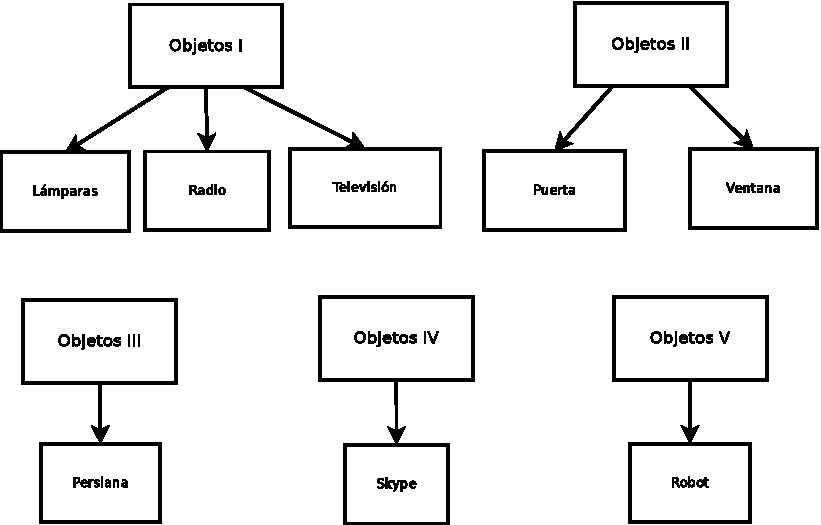
\includegraphics{Esquema_objetos}
  \caption{Clasificación de los objetos para la gramática (aquí también
    se pueden poner acrónimos como \acs{ETTS} y símbolos como \ac{xidet})}
  \label{fig:fig_clobj}
\end{figure}


\subsection{Definición y uso de acrónimos (aquí también
  se pueden poner acrónimos como \acs{ETTS})}
\label{sec:uso-de-acronimos}

El uso del paquete \texttt{glossaries} permite definir los acrónimos y
el sistema automáticamente gestiona su inclusión completa la primera vez
que se usa. Los acrónimos de ejemplo están en el fichero
\texttt{acronyms/defacronymsgl.tex} (con opciones adicionales de
configuración en \texttt{acronyms/acronymsgl.tex}).

Así, si nos referimos a \ac{ETTS} o bien a \ac{EMODB},
veremos como aparecen expandidas la primera vez. A partir de ahí, sólo
se usará el acrónimo como puede verse al volver a hablar de \ac{ETTS} y
\ac{EMODB}.

Tiene también soporte para resetear todos los acrónimos como si no
estuvieran usados. Vuelvo a incluir el párrafo anterior tras un reset
(que se hace con un \texttt{\textbackslash{}glsresetall[acronym]}):

\glsresetall[acronym]

El uso del paquete acronym permite definir los acrónimos y el sistema
automáticamente gestiona su inclusión completa la primera vez que se
usa. Así, si nos referimos a \ac{ETTS} o bien a \ac{EMODB}, veremos como
aparecen expandidas de nuevo (como si fuera la primera vez que se
usan). A partir de ahí, sólo se usará el acrónimo como puede verse al
volver a hablar de \ac{ETTS} y \ac{EMODB}.

Y permite también forzar que se vuelva a citar completo aunque ya se
haya utilizado (con el acrónimo entre paréntesis), como puede verse en
\acl{ETTS} (equivalente a \glsdesc{ETTS} que vale para cualquier
glosario), y también a usar forzosamente el acrónimo. Primero reseteamos
de nuevo.

\glsresetall[acronym]

Y ahora forzamos el acrónimo: \acs{EMODB} (equivalente a
\glsname{EMODB} que vale para cualquier glosario). También podemos
forzar a que lo ponga todo, con \acf{EMODB}.


Podemos seguir definiendo entradas de acrónimos, referirnos a \ac{DBN}
por primera vez, y las siguientes aparecerá como \ac{DBN}.  Pongo ahora
el resto de acrónimos \ac{SQ}, \ac{EIR}, \ac{SIR} y
\ac{ES}. Finalmente los repito para que se vea el efecto: \ac{SQ},
\ac{EIR}, \ac{SIR} y \ac{ES}.

Y gestiona bien los plurales, ponemos el plural como \acp{SOC} la
primera vez, y luego la segunda como \acp{SOC}. Y podemos volver al
singular con \ac{SOC}.


\subsection{Definición y uso de símbolos (aquí también
  se pueden símbolos como \ac{xidet})}
\label{sec:simbolos}

Los símbolos definidos están incluidos en el fichero
\texttt{symbols/defsymbolsgl.tex} (con configuración adicional en
\texttt{symbols/symbolsgl.tex}) y en esta sección mostramos algunos
ejemplos.

El \ac{angstrom} se usa en biología estructural, mientras que el
\ac{ohm} se usa en electrónica. También podemos poner~\ac{xdet}. Y




%%% Local Variables:
%%% TeX-master: "../book"
%%% End:


